\title{COMP3702 - Assignment 2}
\author{Roy Portas - 43560846}
\date{\today}

\documentclass[12pt]{article}
\usepackage{graphicx}
\usepackage{geometry}
\usepackage{listings}
\geometry{
    a4paper,
    margin=1in
}

\begin{document}
    \maketitle

    \section{Chosen Configuration Space}

    The chosen configuration space will be the area containing all valid chair movements. Below is an example of what the configuration space will look like.

    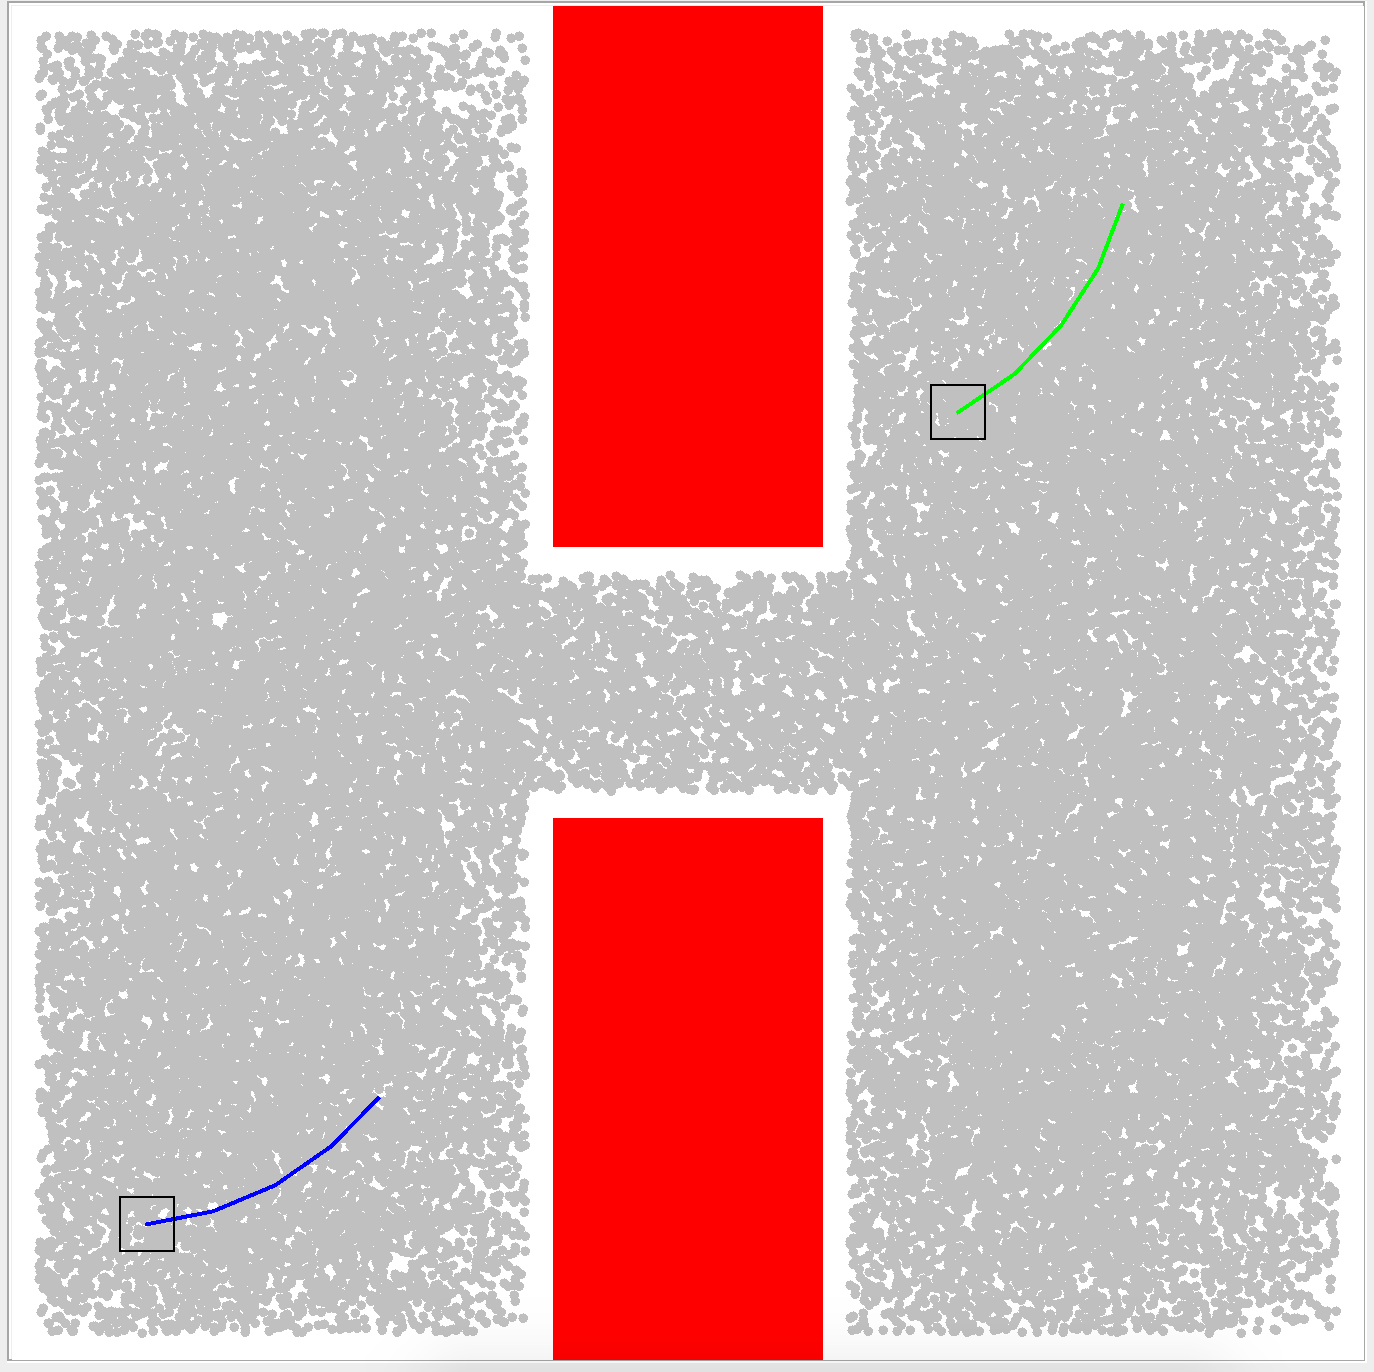
\includegraphics[scale=0.5]{resources/c-space.png}

    In the image above, the grey dots are the chair basepoints generated by the sampling strategy. It can be seen that the border of the grey area will be the configuration space, as the area outside of it is invalid for the chair to move.

    \section{Sampling Strategy}

    There are various sampling strategies that could work for the given problem, most notably:

    \begin{itemize}
        \item Sampling Near Obstacles
        
            This method is promising, since we are given all the obstacles at the start. Thus this sampling only needs to be done once. Furthermore, sampling near obstacles will reduce the number of nodes required and make the graph more sparse. 
            A large distance between two nodes suggest that the space does not have a collision, so the algorithm can move the chair in a straight line towards the node.
            Upon reaching a more dense section of the graph, the algorithm will use the nodes near obstacles to navigate around it.

        \item Sample Inside a Passage

            The obstacles for our problem can be sparse, with large distances between obstacles. Thus this strategy would not be an optimal choice.

        \item Using Workspace Information

            This strategy also looks promising, as we are given the complete workspace. Thus a possible solution is to sample the workspace randomly to create a discrete grid. However this will create a lot of nodes, which will slow down the search algorithm.
            Furthermore, this sampling strategy will create nodes in the empty spaces in the corners of the workspaces, these nodes are irrelevant and will only slow the search algorithm.
    \end{itemize}

    A combination of the Sampling Near Obstacles and 

    \subsection{Implementation}

    The strategy was implemented using the following pseudocode:

    \begin{lstlisting}
        N = Number of required samples
        samples = List of valid samples

        while samples.length < N:
            
            x = Random configuration near an obstacle
            if x is a valid configuration:
                add x to samples

    \end{lstlisting}

    The end result of this will be a list of valid configurations in the workspace.

    \section{What will cause the program to succeed}

    In theory as long as there is a number of valid configurations between the start and destination, the program will succeed. However the chances are increased if the number of samples is larger.

    \section{What will cause the program to fail}

    The program will fail if the number of samples is insufficient. Furthermore, since it depends on sampling near obstacles, if the obstacles are too close together the sampling will fail.
\end{document}
